\documentclass[11pt]{article}
\usepackage[top=1cm, bottom=2cm, left=1cm, right=1cm]{geometry}
\usepackage{ctex}
\usepackage{algorithm}
\usepackage{algorithmicx}
\usepackage{algpseudocode}
\usepackage{amsthm,amsmath,amssymb}
\usepackage[colorlinks=true,linkcolor=blue]{hyperref}
\usepackage{listings}
\usepackage{xcolor,xparse}
\usepackage{realboxes}
\usepackage{graphics}
\usepackage{graphicx}
\usepackage{mathrsfs}
\usepackage{wrapfig}
\usepackage{subfigure}
\usepackage{pifont}
\newcommand{\To}{\textbf{To} }
\definecolor{cmdbg}{rgb}{0.9,0.9,0.9}
\lstset{%
	basicstyle=\ttfamily,
	breaklines = true,
	backgroundcolor=\color{cmdbg},
}
\DeclareDocumentCommand{\ccmd}{v}{% 参数 v 表示工作方法类似于 \verb
    \Colorbox{cmdbg}{\csname lstinline\endcsname!#1!}%
}

\makeatletter
\newenvironment{breakablealgorithm}
  {% \begin{breakablealgorithm}
   \begin{center}
     \refstepcounter{algorithm}% New algorithm
     \hrule height.8pt depth0pt \kern2pt% \@fs@pre for \@fs@ruled
     \renewcommand{\caption}[2][\relax]{% Make a new \caption
       {\raggedright\textbf{\ALG@name~\thealgorithm} ##2\par}%
       \ifx\relax##1\relax % #1 is \relax
         \addcontentsline{loa}{algorithm}{\protect\numberline{\thealgorithm}##2}%
       \else % #1 is not \relax
         \addcontentsline{loa}{algorithm}{\protect\numberline{\thealgorithm}##1}%
       \fi
       \kern2pt\hrule\kern2pt
     }
  }{% \end{breakablealgorithm}
     \kern2pt\hrule\relax% \@fs@post for \@fs@ruled
   \end{center}
  }
\makeatother

\author{谢昀城 22307110070}
\title{计算物理作业3}

\begin{document}
\maketitle


\section{题目1:牛顿法插值和三次样条插值}
\subsection{题目描述}
Newton interpolation of:
\begin{enumerate}
    \item 10 equal spacing points$cos(x),x\epsilon[0,\pi]$
    \item 10 equal spacing points${1\over (1+25 x^2)},x\epsilon [-1,1]$
\end{enumerate}
Compare the results with the cubic spline interpolation.
\subsection{程序描述}
  本程序中,我们将首先使用递归的方法计算$f[x_0,...x_n]={f[x_1,...x_n]-f[x_0,...x_{n-1}]\over x_n-x_0}$,得到Newton插值系数,并还原出插值函数,在程序中由f,Newton\_coefficients,Newton\_interpolatefunc三个函数实现。
  
  对于三次样条差值,我们通过求解以下n-2个线性方程组得到$f''(x_i)$,并还原出插值函数,于函数splines\_funciton中实现,其中求解线性方程组的部分,由homework3中的guaussian\_elimination函数,通过高斯消元法实现。
  \begin{align*}
    \left(x_i - x_{i-1}\right) f''(x_{i-1}) 
    &+ 2\left(x_{i+1} - x_{i-1}\right) f''(x_i) 
    + \left(x_{i+1} - x_i\right) f''(x_{i+1}) \notag \\
    &= \frac{6}{x_{i+1} - x_i} \left[ f(x_{i+1}) - f(x_i) \right] 
    + \frac{6}{x_i - x_{i-1}} \left[ f(x_i) - f(x_{i-1}) \right], \quad i = 2, \dots, n-1
\end{align*}

  $$
  f''(x_1) = f''(x_n) = 0
  $$

  本程序源文件为Interpolation.py,在终端进入当前目录,使用命令python -u Interpolation.py运行本程序。运行时请保证Python第三方库Numpy,Matplotlib已安装,并且与gaussian\_elimination.py置于同一文件下。程序开发环境为Python3.12.3,可在Python3.8以上版本中运行。


\subsection{伪代码} 
\subsubsection{牛顿法插值伪代码:}
\begin{breakablealgorithm}
  \caption{f}
  \begin{algorithmic}
    \Function{f}{$xl, yl$}
      \State \textbf{INPUT:} $xl$ (array of x values), $yl$ (array of y values)
      \State \textbf{OUTPUT:} f[xl](float)

      \If {length($xl$) = 1}
        \State \Return $yl[0]$
      \Else
        \State \Return $\left(f(xl[1:], yl[1:]) - f(xl[0:-1], yl[0:-1])\right) / (xl[-1] - xl[0])$
      \EndIf
    \EndFunction
  \end{algorithmic}
  \end{breakablealgorithm}
  
  \begin{breakablealgorithm}
  \caption{NewtonCoefficients}
  \begin{algorithmic}
    \Function{NewtonCoefficients}{$xl, yl$}
      \State \textbf{INPUT:} $xl$ (array of x values), $yl$ (array of y values)
      \State \textbf{OUTPUT:} coefficients (array of Newton coefficients)
      \State \Return [$f(xl[0:n], yl[0:n])$ \text{ for } $n \gets 1$ \To $n$]
    \EndFunction
  \end{algorithmic}
  \end{breakablealgorithm}
  
  \begin{breakablealgorithm}
  \caption{NewtonInterpolateFunc}
  \begin{algorithmic}
    \Function{NewtonInterpolateFunc}{$x, xl, cl$}
      \State \textbf{INPUT:} $x$ (array of interpolation points), $xl$ (array of x values), $cl$ (array of coefficients)
      \State \textbf{OUTPUT:} $y$ (array of interpolated values)
      \State $y \gets \mathbf{zeros}(x.\text{shape})$
      \For{$i \gets 1$ \To \text{length}(cl)}
        \State $y \gets y + cl[i] \times \prod([x - xi \text{ for } xi \in xl[0:i]])$
      \EndFor
      \State \Return $y$
    \EndFunction
  \end{algorithmic}
  \end{breakablealgorithm}

\subsubsection{三次样条插值伪代码:}
\begin{breakablealgorithm}
  \caption{SplinesFunction}
  \begin{algorithmic}
    \Function{SplinesFunction}{$x, x_l, y_l$}
      \State \textbf{INPUT:} $x$ (interpolation point), $x_l$ (array of x values), $y_l$ (array of y values)
      \State \textbf{OUTPUT:} result (float)
      \State $n \gets \text{length}(x_l)$
      \State $A \gets \mathbf{zeros}(n-2, n-2)$
      \State $B \gets \mathbf{zeros}(n-2)$
      
      \For{$i \gets 1$ \To $n-1$}
        \State $A[i-1,i-1] \gets 2 \cdot (x_{i+1} - x_{i-1})$
        \If{$i < n-2$}
          \State $A[i-1,i] \gets x_{i+1} - x_i$
        \EndIf
        \If{$i > 1$}
          \State $A[i-1,i-2] \gets x_i - x_{i-1}$
        \EndIf
        \If{$i > 1$ \textbf{and} $i < n-2$}
          \State $B[i-1] \gets 6 \cdot \left(\frac{y_{i+1} - y_i}{x_{i+1} - x_i}\right) + 6 \cdot \left(\frac{y_{i-1} - y_i}{x_i - x_{i-1}}\right)$
        \EndIf
      \EndFor
  
      \State $B[0] \gets 6 \cdot \left(\frac{y_2 - y_1}{x_2 - x_1}\right) + 6 \cdot \left(\frac{y_0 - y_1}{x_1 - x_0}\right)$
      \State $B[-1] \gets 6 \cdot \left(\frac{y_{n-1} - y_{n-2}}{x_{n-1} - x_{n-2}}\right) + 6 \cdot \left(\frac{y_{n-3} - y_{n-2}}{x_{n-2} - x_{n-3}}\right)$
      
      \State $M \gets \mathbf{hstack}(A, B.\text{reshape}(-1, 1))$
      \State $cl \gets$ $\mathbf{hstack}$(0,GaussianElimination($M$).0)
    
      \For{$i \gets 1$ \To $n$}
        \If{$x_{i-1} \leq x \leq x_i$}
          \State \Return $cl[i-1] \cdot \frac{(x_i - x)^3}{6 \cdot (x_i - x_{i-1})} + cl[i] \cdot \frac{(x - x_{i-1})^3}{6 \cdot (x_i - x_{i-1})} + \left(\frac{y_{i-1}}{x_i - x_{i-1}} - cl[i-1] \cdot \frac{x_i - x_{i-1}}{6}\right) \cdot (x_i - x) + \left(\frac{y_i}{x_i - x_{i-1}} - cl[i] \cdot \frac{x_i - x_{i-1}}{6}\right) \cdot (x - x_{i-1})$
        \EndIf
      \EndFor
    \EndFunction
  \end{algorithmic}
  \end{breakablealgorithm}

  \subsection{输入输出实例}
  对于本程序,运行后将生成$cos(x)$和${1\over 1+25 x^2}$的插值结果为Interpolation1.png和Interpolation2.png,于当前目录下,如图\ref{fig:1}和\ref{fig:2}所示,并计算牛顿差值和三次样条差值的平均平方误差,程序运行截图如图\ref{fig:3}所示。可以看到,对于$cos(x)$,两种插值方法效果均较好,牛顿法的误差比样条法更小。而对于${1\over 1+25x^2}$,牛顿法对于中心区域的插值效果比样条法好,但是在远离原点处产生了不存在的振荡,并且在超出插值范围后迅速增大,而样条法在远离原点处的效果较好。

  \begin{figure}[ht]
    \centering
    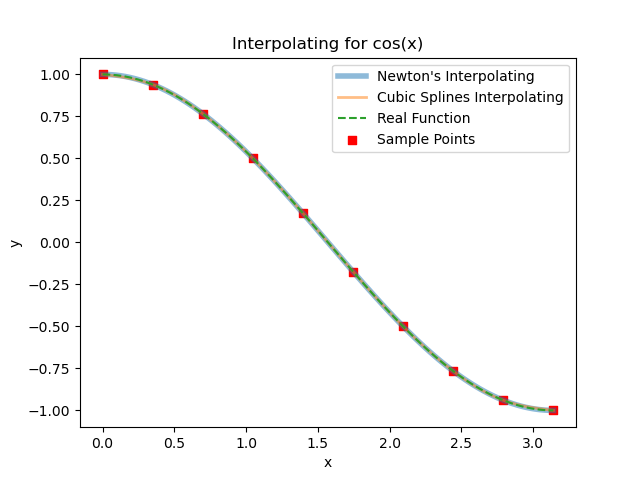
\includegraphics[width=0.6\linewidth]{photo/Interpolation1.png}
    \caption{Cos(x)插值}
    \label{fig:1}
  \end{figure}

  \begin{figure}[ht]
    \centering
    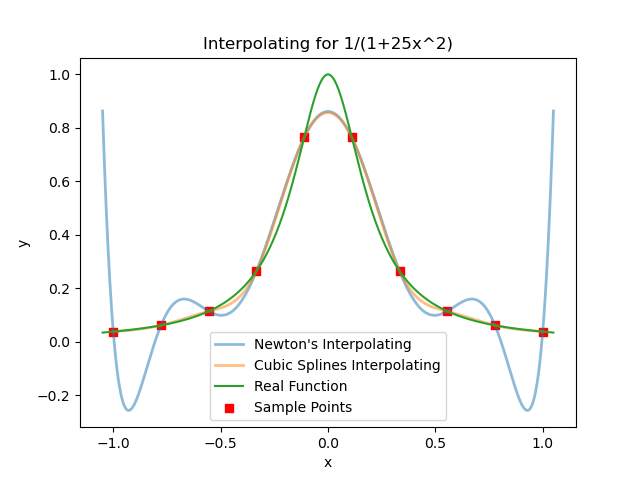
\includegraphics[width=0.6\linewidth]{photo/Interpolation2.png}
    \caption{$1/(1+25x^2)$插值}
    \label{fig:2}
  \end{figure}
  \begin{figure}[ht]
    \centering
    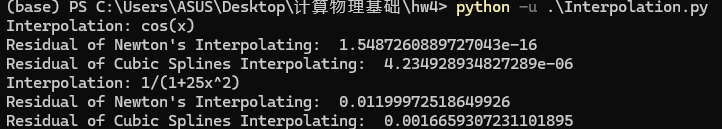
\includegraphics[width=0.6\linewidth]{photo/fig1.png}
    \caption{题目1程序运行截图}
    \label{fig:3}
  \end{figure}

  \section{题目3}
  \subsection{题目描述}
  The table below gives the temperature 
 along a metal rod whose ends are kept at fixed constant temperatures. The temperature is a function of the distance 
 along the rod.
 \begin{enumerate}
  \item Compute a least-squares, straight-line fit to these data using $T(x)=a+bx$
  \item Compute a least-squares, parabolic-line fit to these data using $T(x)=a+bx+cx^2$
\end{enumerate}
\subsection{程序描述}
在本程序中,我们将通过SVD分解对T-x做线性和二次拟合。即考虑:$A=(I,x)$和$A=(I,x,x^2)$,$B=T$,求解$A\beta=B$。其中SVD分解使用numpy库的np.linalg.svd函数实现


本程序源文件为least\_square.py,在终端进入当前目录,使用命令python -u least\_square.py运行本程序。运行时请保证Python第三方库Numpy,Matplotlib已安装。程序开发环境为Python3.12.3,可在Python3.8以上版本中运行。

\subsection{伪代码}
\subsubsection{Trapezoidal integrate 伪代码:}

\begin{breakablealgorithm}
  \caption{LeastSquarebySVD}
  \begin{algorithmic}

      $A\gets(1,x)$ or $(1,x,x^2)$

      $U,S,V\gets SVD(A)$

      $\beta\gets V S^{-1} U^T B$

      \textbf{Return} $\beta$
  \end{algorithmic}
  \end{breakablealgorithm}
  
  
  \subsection{输入输出实例}
  对于本程序,运行后会生成线性和二次拟合曲线图\ref{fig:4},"least\_square.png"于当前目录下,并输出最小平方距离和$R^2$,程序运行截图为图\ref{fig:5},得到:

  Straight-line fit:$T = 0.889 + 10.073x,Least squares:380.96,R^2 = 0.9$

  Quadratic-line fit:$T = 8.262 + 6.052x + 0.402x^2,Least squares:331.145,R^2 = 0.95$

  
 
  \begin{figure}[ht]
    \centering
    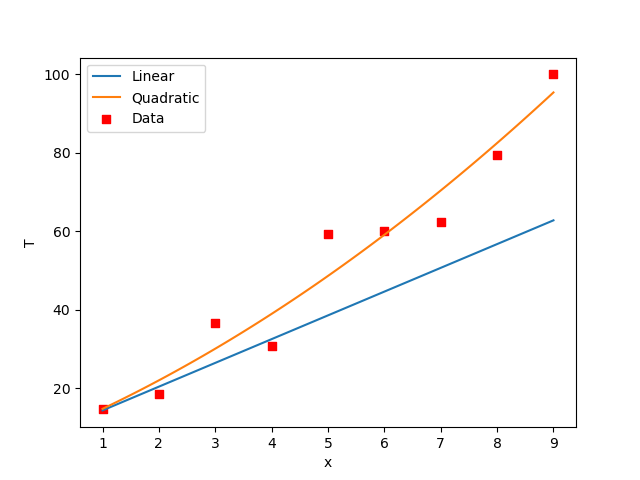
\includegraphics[width=0.8\linewidth]{photo/least_square.png}
    \caption{拟合曲线}
    \label{fig:4}
  \end{figure}



  \begin{figure}
    \centering
    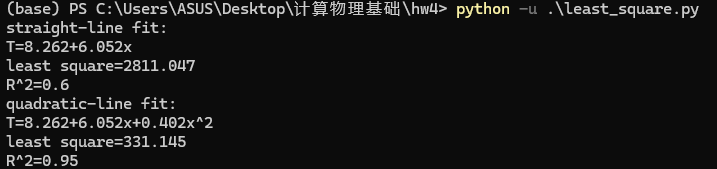
\includegraphics[width=0.6\linewidth]{photo/fig2.png}
    \caption{题目2程序运行截图}
    \label{fig:5}
  \end{figure}

  

\end{document}


